\subsection{Motivating Example}\label{example} 

\begin{figure}[!h]
\begin{center}
\EmbedCode{c}{main.c}{left}
\end{center}
\caption{Motivating Example}
\label{fig:sample}
\end{figure}

Figure~\ref{fig:sample} shows $4$ C functions:
\main, \even, \odd, and \compute.

In \main{}, function \texttt{scanf} from the standard input/ouput
library gets an integer input from user at line $3$
and stores it in variable \texttt{x}. \texttt{x} 
becomes \textit{tainted} since it holds a value from
the environment which has not been validated and
sanitized.
\texttt{x} is later used in line $4$ as argument to \even{}
and at line $6$ as argument to \odd{}.

In \compute{}, variable \texttt{sum} gets tainted at
line $13$ through function \texttt{scanf}. Variable
\texttt{x} is tainted only if it was passed tainted
at calling sites.

In functions \even{}, and \odd{}, variable \texttt{x}
is tainted only when it has been passed as tainted
at calling sites.

\begin{comment}
\begin{figure}
\begin{minipage}[b]{0.45\textwidth}
	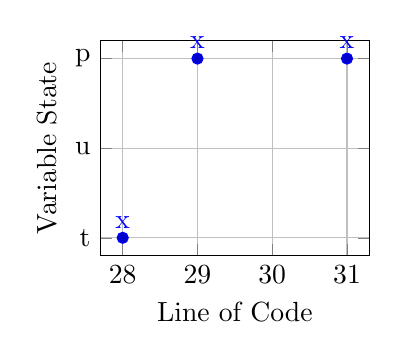
\begin{tikzpicture}
		\begin{axis}[
					 xlabel=Line of Code,					 
					 symbolic y coords={t,u,p},		
					 ylabel=Variable State,				
					 ytick={t,u,p},
					 xtick={28,29, ...,31},
					 grid=both,
					 width=5cm				 
					 ]				 
			\addplot+ [only marks,
					   nodes near coords=x ] coordinates {
				(28,t)
				(29,p)
				(31,p)
				};
		\end{axis}
	\end{tikzpicture}	
	\caption{Taint Information for \main{}}\label{fig:taintmain}
	\end{minipage}		
	\begin{minipage}[b]{0.45\textwidth}
	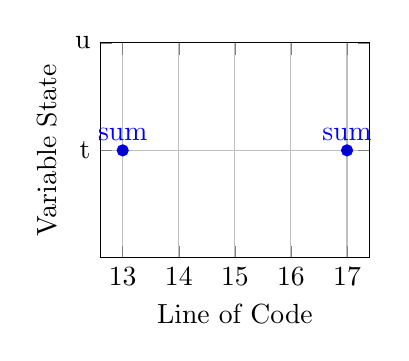
\begin{tikzpicture}
		\begin{axis}[
					 xlabel=Line of Code,					 
					 symbolic y coords={t,u,p},		
					 ylabel=Variable State,				
					 ytick={t,u,p},
					 xtick={11,12, ...,18},
					 grid=both,
					 width=5cm				 
					 ]				 
			\addplot+ [only marks,
					   nodes near coords=sum ] coordinates {
				(13,t)
				(17,t)				
				};
		\end{axis}
	\end{tikzpicture}	
	\caption{Taint Information for \compute{}}\label{fig:taintcompute}
	\end{minipage}			
\end{figure}
\end{comment}

\subsection{Handling of complex data structures}
